%% LyX 2.1.2.1 created this file.  For more info, see http://www.lyx.org/.
%% Do not edit unless you really know what you are doing.
\documentclass[english]{beamer}
\usepackage[T1]{fontenc}
\usepackage[latin9]{inputenc}
\setcounter{secnumdepth}{3}
\setcounter{tocdepth}{3}
\usepackage{amsmath}
\usepackage{amssymb}
\usepackage{graphicx}

\makeatletter
%%%%%%%%%%%%%%%%%%%%%%%%%%%%%% Textclass specific LaTeX commands.
 % this default might be overridden by plain title style
 \newcommand\makebeamertitle{\frame{\maketitle}}%
 % (ERT) argument for the TOC
 \AtBeginDocument{%
   \let\origtableofcontents=\tableofcontents
   \def\tableofcontents{\@ifnextchar[{\origtableofcontents}{\gobbletableofcontents}}
   \def\gobbletableofcontents#1{\origtableofcontents}
 }

%%%%%%%%%%%%%%%%%%%%%%%%%%%%%% User specified LaTeX commands.
\beamertemplateshadingbackground{red!5}{structure!5}

\usepackage{beamerthemeshadow}
\usepackage{pgfnodes,pgfarrows,pgfheaps}

\beamertemplatetransparentcovereddynamicmedium






\newcommand{\Class}[1]{\operatorname{\mathchoice
  {\text{\small #1}}
  {\text{\small #1}}
  {\text{#1}}
  {\text{#1}}}}

\newcommand{\Lang}[1]{\operatorname{\text{\textsc{#1}}}}

\newcommand{\tape}[3]{%
  \color{structure!30!bg}
  \pgfmoveto{\pgfxy(-0.5,0)}
  \pgflineto{\pgfxy(-0.6,0.1)}
  \pgflineto{\pgfxy(-0.4,0.2)}
  \pgflineto{\pgfxy(-0.6,0.3)}
  \pgflineto{\pgfxy(-0.4,0.4)}
  \pgflineto{\pgfxy(-0.5,0.5)}
  \pgflineto{\pgfxy(4,0.5)}
  \pgflineto{\pgfxy(4.1,0.4)}
  \pgflineto{\pgfxy(3.9,0.3)}
  \pgflineto{\pgfxy(4.1,0.2)}
  \pgflineto{\pgfxy(3.9,0.1)}
  \pgflineto{\pgfxy(4,0)}
  \pgfclosepath
  \pgffill

  \color{structure}  
  \pgfputat{\pgfxy(0,0.7)}{\pgfbox[left,base]{#1}}
  \pgfputat{\pgfxy(0,-0.1)}{\pgfbox[left,top]{#2}}

  \color{black}
  \pgfputat{\pgfxy(-.1,0.25)}{\pgfbox[left,center]{\texttt{#3}}}%
}

\newcommand{\shorttape}[3]{%
  \color{structure!30!bg}
  \pgfmoveto{\pgfxy(-0.5,0)}
  \pgflineto{\pgfxy(-0.6,0.1)}
  \pgflineto{\pgfxy(-0.4,0.2)}
  \pgflineto{\pgfxy(-0.6,0.3)}
  \pgflineto{\pgfxy(-0.4,0.4)}
  \pgflineto{\pgfxy(-0.5,0.5)}
  \pgflineto{\pgfxy(1,0.5)}
  \pgflineto{\pgfxy(1.1,0.4)}
  \pgflineto{\pgfxy(0.9,0.3)}
  \pgflineto{\pgfxy(1.1,0.2)}
  \pgflineto{\pgfxy(0.9,0.1)}
  \pgflineto{\pgfxy(1,0)}
  \pgfclosepath
  \pgffill

  \color{structure}  
  \pgfputat{\pgfxy(0.25,0.7)}{\pgfbox[center,base]{#1}}
  \pgfputat{\pgfxy(0.25,-0.1)}{\pgfbox[center,top]{#2}}

  \color{black}
  \pgfputat{\pgfxy(-.1,0.25)}{\pgfbox[left,center]{\texttt{#3}}}%
}

\pgfdeclareverticalshading{heap1}{\the\paperwidth}%
  {color(0pt)=(black); color(1cm)=(structure!65!white)}
\pgfdeclareverticalshading{heap2}{\the\paperwidth}%
  {color(0pt)=(black); color(1cm)=(structure!55!white)}
\pgfdeclareverticalshading{heap3}{\the\paperwidth}%
  {color(0pt)=(black); color(1cm)=(structure!45!white)}
\pgfdeclareverticalshading{heap4}{\the\paperwidth}%
  {color(0pt)=(black); color(1cm)=(structure!35!white)}
\pgfdeclareverticalshading{heap5}{\the\paperwidth}%
  {color(0pt)=(black); color(1cm)=(structure!25!white)}
\pgfdeclareverticalshading{heap6}{\the\paperwidth}%
  {color(0pt)=(black); color(1cm)=(red!35!white)}

\newcommand{\heap}[5]{%
  \begin{pgfscope}
    \color{#4}
    \pgfheappath{\pgfxy(0,#1)}{\pgfxy(-#2,0)}{\pgfxy(#2,0)}
    \pgfclip
    \begin{pgfmagnify}{1}{#1}
      \pgfputat{\pgfpoint{-.5\paperwidth}{0pt}}{\pgfbox[left,base]{\pgfuseshading{heap#5}}}
    \end{pgfmagnify}
  \end{pgfscope}
  %\pgffill
  
  \color{#4}
  \pgfheappath{\pgfxy(0,#1)}{\pgfxy(-#2,0)}{\pgfxy(#2,0)}
  \pgfstroke

  \color{white}
  \pgfheaplabel{\pgfxy(0,#1)}{#3}%
}


\newcommand{\langat}[2]{%
  \color{black!30!beamerexample}
  \pgfsetlinewidth{0.6pt}
  \pgfsetendarrow{\pgfarrowdot}
  \pgfline{\pgfxy(-3.5,#1)}{\pgfxy(0.05,#1)}
  \color{beamerexample}
  \pgfputat{\pgfxy(-3.6,#1)}{\pgfbox[right,center]{#2}}%
}

\newcommand{\langatother}[2]{%
  \color{black!30!beamerexample}
  \pgfsetlinewidth{0.6pt}
  \pgfsetendarrow{\pgfarrowdot}
  \pgfline{\pgfxy(3.5,#1)}{\pgfxy(-0.05,#1)}
  \color{beamerexample}
  \pgfputat{\pgfxy(3.6,#1)}{\pgfbox[left,center]{#2}}%
}


\pgfdeclaremask{knight1-mask}{beamer-knight1-mask} \pgfdeclareimage[height=2cm,mask=knight1-mask]{knight1}{beamer-knight1} \pgfdeclaremask{knight2-mask}{beamer-knight2-mask} \pgfdeclareimage[height=2cm,mask=knight2-mask]{knight2}{beamer-knight2} \pgfdeclaremask{knight3-mask}{beamer-knight3-mask} \pgfdeclareimage[height=2cm,mask=knight3-mask,interpolate=true]{knight3}{beamer-knight3} \pgfdeclaremask{knight4-mask}{beamer-knight4-mask} \pgfdeclareimage[height=2cm,mask=knight4-mask,interpolate=true]{knight4}{beamer-knight4}


\pgfdeclareradialshading{graphnode}
  {\pgfpoint{-3pt}{3.6pt}}%
  {color(0cm)=(beamerexample!15);
    color(2.63pt)=(beamerexample!75);
    color(5.26pt)=(beamerexample!70!black);
    color(7.6pt)=(beamerexample!50!black);
    color(8pt)=(beamerexample!10!bg)}

\newcommand{\graphnode}[2]{
  \pgfnodecircle{#1}[virtual]{#2}{8pt}
  \pgfputat{#2}{\pgfbox[center,center]{\pgfuseshading{graphnode}}}
}

\makeatother

\usepackage{babel}
\begin{document}

\title{Correlated Multi-armed Bandits}


\subtitle{CS 6780 Advanced Machine Learning}


\author{Zhengdi Shen\\
Bangrui Chen\\
Saul Toscano Palmerin}


%\institute{Cornell University\\
%\includegraphics[scale=0.04]{../../../../q-exam/cornell}\\
%}


\date{April 23, 2015}
\makebeamertitle
\begin{frame}{Motivation}

\begin{block}{}


For a new user on Yelp, what restaurants should Yelp recommend at
each time to maximize the expected average rating of the user?\\
\textrm{}\\


\begin{itemize}
\item Each restaurant is represented with a $r$ dimensional binary vector, corresponding to the categories it belongs to
(e.g. Pizza, Sandwiches, Mexican, Chinese, Italian).\\
\textrm{}\\
\item Each user has an unknown preference vector $\theta$.\\
% Difficulty in large number of arms
% n categories -> at most 2^n arms
\textrm{}\\
\item Multi-Armed Bandits.
(At most $2^r$ arms!)\\
\textrm{}\\
\item Dependent arms.
% Correlation between different restaurants
\end{itemize}
\end{block}
\end{frame}

\begin{frame}{Motivation}
\begin{table}
\centering
\begin{tabular}{|c|c|c|c|c|c|}
\hline
$r=5$ & Pizza & Sandwiches & Mexican & Chinese & Italian  \\ \hline
 Restaurant 1 & 1 & 1 & 1 & 0 & 1 \\ \hline
 Restaurant 2 & 1 & 1 & 0 & 0 & 1 \\ \hline
 Restaurant 3 & 0 & 0 & 0 & 1 & 0 \\ \hline
  Restaurant 4 & 1 & 0 & 0 & 0 & 1 \\ \hline
 $\cdots$ & $\cdots$ & $\cdots$ & $\cdots$ & $\cdots$ & $\cdots$ \\ \hline
\end{tabular}
\end{table}

\end{frame}

\begin{frame}{Problem Formulation}

\begin{block}{}

\begin{itemize}
\item The reward of choosing a restaurant with features $X\in\left\{ 0,1\right\} ^{r}$
at time $t$ is defined by
\[
Y_{t}=X\cdot\theta+W_{t}
\]
where $W_{t}\sim N\left(0,\sigma^{2}\right)$ is a measurement error.\\
\textrm{}\\
\item We place a Gaussian prior distribution on the preference vector: $\theta$
$\sim N\left(\mu_{0},\Sigma_{0}\right)$\\
\textrm{}\\
\end{itemize}
\end{block}
\end{frame}

\begin{frame}{Regret}





\begin{block}{Definition of Regret}


For any policy, we define the T-period regret cumulative as
\[
\mbox{Regret}\left(\theta_{0},T\right)=\sum_{t=1}^{T}\mathbb{E}\left[\mbox{max}_{X\in\left\{ 0,1\right\} ^{r}}X\cdot\theta_{0}-X_{t}\cdot\theta_{0}\mid\theta=\theta_{0}\right]
\]
where $X_{t}$ is the feature vector of the restaurant selected at
stage $t$.

\end{block}
\end{frame}

\begin{frame}{Lower Bound for Regret}





\begin{block}{Lower Bound for Regret}


For an arbitrary policy, the regret is at least $\varOmega\left(r\sqrt{T}\right)$
under some regularity conditions, where the set of arms is compact
in $\mathbb{R}^{r}$.

\end{block}
\end{frame}

\begin{frame}{``Optimal Algorithm''}




The Phased Exploration and Greedy Exploitation (PEGE) algorithm has
regret $\varOmega\left(r\sqrt{T}\right)$ under some regularity conditions.
\\

\pause{}
\textrm{}\\


\begin{block}{PEGE \quad [ Linearly Parameterized Bandits, P. R., J. T., 2010]}
Find $r$ arms $X_{b_1},\cdots, X_{b_r}$ which form a maximal linearly independent system.

In each cycle $c$:
\begin{enumerate}
\item Exploration (r periods): Play arm $X_{b_k}$, and observe
the reward $Y^{X_{b_k}}\left(c\right)$. Compute the ordinary least
squares estimate $\hat{\theta}\left(c\right)$. \\
\textrm{}\\
\item Exploitation (c periods): Play the greedy arm $G\left(c\right)=\mbox{arg max}_{X}X\cdot\hat{\theta}\left(c\right)$\inputencoding{latin1}{
for $c$}\inputencoding{latin9} periods.\\
\textrm{}\\
\end{enumerate}
\end{block}
\pause{}

But it may have large constant in front of the order of its regret.

\end{frame}

\begin{frame}{``Optimal Algorithm''}
\begin{figure}
\centering
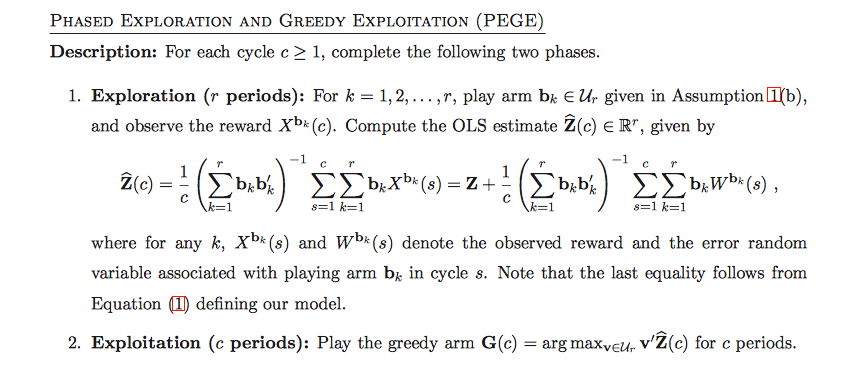
\includegraphics[scale=0.35]{PEGE.png}
\end{figure}
\end{frame}




\begin{frame}{Exponentiated Gradient Algorithm (EGA)}


\begin{block}{EGA}



\begin{figure}
\centering
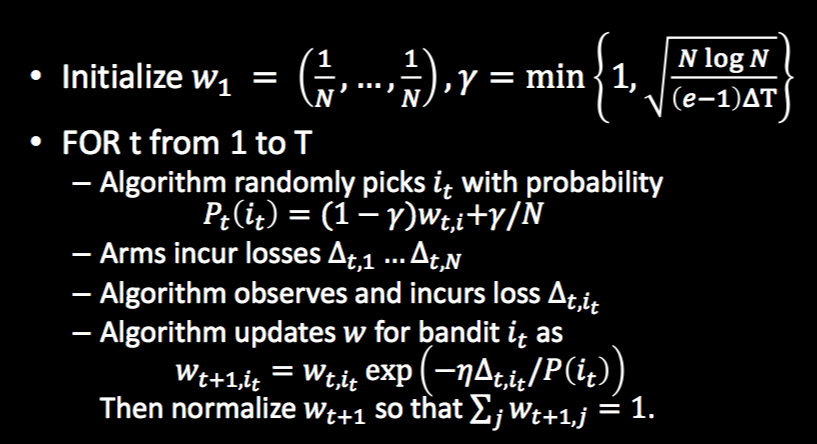
\includegraphics[scale=0.3]{EGA.png}
\end{figure}

\end{block}

\end{frame}





\begin{frame}{Upper Confidence Bound (UCB)}



\begin{block}{UCB}




Given $\theta\sim N\left(\mu_{0},\Sigma_{0}\right)$, for $t$ from
$1$ to $T$:
\begin{enumerate}
\item Play arm $X_{i_{t}}=\mbox{arg max}\left\{ \mu_{t-1}\cdot X_{i}+1.96X_{i}'\sum_{t-1}X_{i}\right\} $
\\
\textrm{}\\
\item Calculate $\mu_{t}$ and $\Sigma_{t}$ based on reward $Y_{t}$, arm
$X_{i_t}$, $\mu_{t-1}$, and $\Sigma_{t-1}$. \\
\textrm{}\\
\end{enumerate}
\begin{figure}
\centering
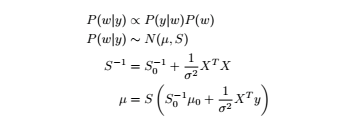
\includegraphics[scale=0.6]{UCB.png}
\end{figure}

\end{block}

\end{frame}



\begin{frame}{Our Goal}

\begin{block}

\begin{itemize}
\item Evaluate the performance of the existing approaches.

\item Develop hybrid methods for specific conditions.

\item Find a way to map the user's rating to a compact set, say integers from 0 to 5.

\end{itemize}

\end{block}

\end{frame}


\begin{frame}




{\Huge{}Thanks!!}{\Huge \par}

{\Huge{}Any Questions?}{\Huge \par}



\end{frame}

\end{document}
